\documentclass[11pt]{article}

\usepackage{booktabs}

\usepackage{geometry}
\geometry{a4paper, margin=2cm, top=1cm}

\usepackage{hyperref}

\usepackage{graphicx}
\usepackage{subcaption}

\begin{document}

\begin{titlepage}
    \vspace*{\fill}    
    \begin{center}
        {\Huge \textbf{Predictive modeling of hospital admission categories: A nominal multimodal approach}} \\[1cm]
    \end{center}
    \vspace*{\fill} 
\end{titlepage}

\newpage
\begin{center}
\section*{
        Executive Summary
}
\end{center}

\subsection*{
    Introduction
    \vspace{-0.25cm}
}
Hospital admission category predictions are important because they can help optimise resource allocation, improve patient flow, and ensure that hospitals are equipped to handle the specific needs of their patients, whether elective, urgent, or emergency. By anticipating admission types, healthcare systems can better plan staffing, prioritise critical cases, and reduce delays in treatment. I create a nominal multimodal to predict the admissions category of a patient using information about the clinical case (length of stay and mortality), their demography (skin colour and age), and characteristics of the hospital they entered.

\vspace{-0.5cm}
\subsection*{
    \vspace{-0.25cm}
    Methods
}
A nominal multimodal model is a statistical tool used to understand and predict outcomes that fall into multiple categories without any natural order. This model particularly suits our case because admissions categories are distinct with no ranking, and the factors influencing them vary in complex ways.

After aggregating data by hospital, I found that the median hospital had zero emergency admissions, and zero admissions of anyone below the age of 44 (categories 1-2) or above the age of 90 (category 9). Some hospitals in the dataset my lack emergency, urgent referrals, pediatric or youth care departments so may not be able to admit these kinds of patients. I account for these differences in hospitals by indirectly inferring hospital characteristics, but this process is an approximation and should be replaced with direct data on hospitals or department availability. I improve on this initial model by adding more terms to better represent hospital characteristics, and remove age as a predictor after determining it to be insignificant.

Furthermore, this analysis identified the existence of "specialist hospitals" in the dataset - hospitals with only elective (e.g cancer treatment centres), urgent admissions (e.g cardiac care units), or emergency admissions (e.g trauma units). This analysis is unlikely to be useful for these hospitals as they only admit one category of patient, so I exclude them to avoid biasing the dataset.

\vspace{-0.5cm}
\subsection*{
    \vspace{-0.25cm}
    Results
}
A more complicated case, such as a case requiring a longer stay or leading to the death of a patient, decreases the chances of an urgent admission compared to an elective admission. White patients are significantly more likely to be admitted after a GP referral compared to non-white patients. No health or demographic factors significantly change the odds of an emergency admission versus an elective admission (see \ref{tab:final_model_summary}).

Characteristics of the attended hospitals significantly impacts the likelihood of admissions category, but the meaning of these variables is difficult to interpret in isolation.  For example, has\_youth is a dummy variable representing whether the patient's hospital has ever admitted a patient between the ages of 22 to 44 - why this variable significantly increases the odds of an urgent referral is unclear by itself, but likely reflects hospital-specific variations, such as service availability or operational policies, that are not fully captured in the dataset.

\vspace{-0.5cm}
\subsection*{
    \vspace{-0.25cm}
    Conclusion
}

This analysis demonstrates the effect of a given patient's case or demography on the category of stay. Complicated cases, such as those requiring longer hospital stays or resulting in patient death, are less likely to be classified as urgent admissions because urgent admissions are typically associated with immediate but non-complex issues that can be resolved quickly, whereas more severe or prolonged cases may necessitate elective planning. White patients have a significantly higher likelihood of being admitted via a GP referral compared to non-white patients, reflecting racial disparities in access to primary care services or referral practices.

Although all the above effects are significant, this model does little to predict admissions categories as a whole.  The present structure of capturing hospital characteristics is inadequate because it relies solely on inferred characteristics. Direct information regarding hospitals, such as types of wards available, patient capacity and staffing levels, could address this weakness and would be the easiest to collate. As the limited number of clinical and demographic variables already serve as significant predictors of admissions category, collecting more clinical (e.g a patient's existing health conditions) and demographic (e.g socioeconomic status) information about patients could improve this model's predictive capabilities. 





\newpage
\begin{center}
\section*{
    Technical Hand-over document
}
\end{center}

\subsection*{
    \vspace{-0.25cm}
    Introduction
}
I explore using a nominal multinomial model approach to predict the category of a patient's admission using demographic (age, race) and clinical (length of stay, death during stay) data.


\vspace{-0.5cm}
\subsection*{
    \vspace{-0.25cm}
    Data exploration
}
I perform a series of ANOVA tests for continuous variables (length of stay and age category) and $\chi^2$ tests for factor variables (all others) to observe whether these variables significantly varied between admissions category. All clinical variables (length of stay: $p < 0.001$, patient death: $p = 0.002$) and the patient's race ($p = 0.001$) significantly varied between admissions categories, whereas neither the continuous age category ($p = 0.775$) nor the factor age80 ($p = 0.410$) proved significant.

The significant $\chi^2$ test for hospital number ($p < 0.001 $) warranted a hospital aggregation of the data. Many hospitals had zero emergency or urgent admissions, zero admissions for certain age groups or all admissions in one category. Assuming that a hospital with zero admissions lacks a specific department, I add a dummy variable to represent the presence or absence of an urgent admissions, pediatric department, youth, and elderly care departments at each hospital, and replace the hospital number with these dummy variables in the disaggregated dataset. A correlation matrix shows these hospital dummy variables vary between themselves (see \ref{tab:corr_matrix_2}), so I add interaction terms between all variables with a correlation larger than 0.2 to further capture these hospital characteristics and minimise AICc at the expense of multicolinearity and interpretability.

 \vspace{-0.5cm}
\subsection*{
    \vspace{-0.25cm}
    Model selection
}

I perform Type 2 Anova selection of all covariates of this large model to reduce the number of variables and lower AICc. All clinical variables (length of stay: $p < 0.001$, died: $p < 0.001$) and admissions-related  (has\_emergency: $p < 0.001$, has\_urgent: $p < 0.001$) and one age-related (has\_elderly: $p = 0.015$) hospital dummies are identified as significant predictions of admissions category. Some hospital dummy interactions (has\_emergency:has\_youth: $p < 0.001$, has\_youth:has\_elderly: $p = 0.009$) are significant, but the rest are discarded. The remaining age-based department dummy  variables (has\_pediatric: $p = 0.080$, has\_youth: $p = 0.152$) and race (white: $p = 0.081$) only approach significance but I include them as their presence lowers AICc slightly (1588.306 to 1584.423). As expected, age is not found to be significant ($p = 0.659$).

 \vspace{-0.5cm}
\subsection*{
    \vspace{-0.25cm}
    Verifying assumptions and diagnostics
}
 To model data using a nomial multimodal model, observations must come from a multinomial distribution. I estimate three binomial models by treating each admissions category as a success and treating the remaining categories as a failure. All three binomial models (AICc for Elective vs Rest: 1396.090, Emergency vs Rest: 365.889, Urgent vs Rest: 1235.866) significantly outperform the multinomial model (1584.424), even if their residuals-fitted plots indicate these models are unstable (see \ref{fig:fitted_residuals_binomial}). The binomial models' vast improvement over the multinomial model is likely driven by the differing coefficients for the admissions-based hospital dummy variables (see \ref{tab:coeff_differences}). These results suggest that this assumption is violated by the hospital dummy variables, which constrain the results to a more binomial outcome as the odds of some outcomes approach zero (e.g an emergency admission in a hospital without an emergency department). Independence of observations is also violated as patients are likely to visit multiple hospitals and have their medical outcome influenced by them, while the assumption of linearity between covariates and the response variable is violated for several factor variables which fail to show clear separability (see \ref{fig:log_odds_grid}).

Despite a $\chi^2$ test reporting no evidence of a a bad fit ($p = 1.000$), this model explains a relatively low amount of variability between admissions categories (McFadden's pseudo $R^2 = 0.106$). The fitted versus residuals plots shows that the model is biased (see \ref{fig:fitted_observed}). 


 \vspace{-0.5cm}
\subsection*{
    \vspace{-0.25cm}
    Conclusion
}

While the model effectively identifies certain demographic, clinical and hospital characteristics as significant, its overall performance is limited. Significant issues include violations of key independence and linearity assumptions, leading to a model that explains only a small proportion of variability in admissions categories and consistently mis-estimates across all admissions types. For this dataset, binomial models used in this study outperformed the multinomial model by better accounting for the restrictive hospital characteristics, and future work should explore a binomial or stratified modelling framework.

\newpage
\section*{
    Appendix
}

\begin{table}[h!]
\centering
\resizebox{\textwidth}{!}{
\begin{tabular}{lcccccccccc}
\hline
 & died & white & los & age80 & age & has\_emergency & has\_urgent & has\_pediatric & has\_youth & has\_elderly \\
\hline
died           & 1.000 & 0.044 & -0.130 & 0.117 & 0.139 & 0.006 & -0.001 & -0.069 & -0.023 & -0.051 \\
white          & 0.044 & 1.000 & -0.050 & 0.050 & 0.181 & 0.102 & -0.039 & -0.185 & -0.124 & -0.038 \\
los            & -0.130 & -0.050 & 1.000 & -0.025 & -0.037 & -0.026 & 0.004 & 0.009 & 0.038 & 0.020 \\
age80          & 0.117 & 0.050 & -0.025 & 1.000 & 0.743 & 0.001 & 0.013 & -0.043 & -0.060 & 0.016 \\
age            & 0.139 & 0.181 & -0.037 & 0.743 & 1.000 & 0.068 & -0.020 & -0.076 & -0.130 & -0.006 \\
has\_emergency & 0.006 & 0.102 & -0.026 & 0.001 & 0.068 & 1.000 & -0.212 & -0.230 & -0.329 & -0.025 \\
has\_urgent    & -0.001 & -0.039 & 0.004 & 0.013 & -0.020 & -0.212 & 1.000 & 0.096 & 0.321 & -0.053 \\
has\_pediatric & -0.069 & -0.185 & 0.009 & -0.043 & -0.076 & -0.230 & 0.096 & 1.000 & 0.300 & 0.035 \\
has\_youth     & -0.023 & -0.124 & 0.038 & -0.060 & -0.130 & -0.329 & 0.321 & 0.300 & 1.000 & 0.264 \\
has\_elderly   & -0.051 & -0.038 & 0.020 & 0.016 & -0.006 & -0.025 & -0.053 & 0.035 & 0.264 & 1.000 \\
\hline
\end{tabular}
}
\caption{Correlation matrix between all variables in the modified dataset.}
\label{tab:corr_matrix_2}
\end{table}


\begin{table}[h!]
\centering
\begin{tabular}{lrrrr}
\hline
\textbf{Term} & \textbf{Coefficient estimate} & \textbf{Standard error} & \textbf{$z$ value} & \textbf{$p$ value} \\
\hline
(Intercept):1                 & $1.790 \times 10^{01}$ & $1.438 \times 10^{03}$ & NA     & NA         \\
(Intercept):2                 & $-1.693$              & $2.133 \times 10^{03}$ & $-0.001$ & 0.999367   \\
los:1                         & $-4.315 \times 10^{-02}$ & $9.679 \times 10^{-03}$ & $-4.459$ & \textbf{8.25e-06} \\
los:2                         & $-2.093 \times 10^{-02}$ & $2.217 \times 10^{-02}$ & $-0.944$ & 0.345049   \\
died1:1                       & $-3.976 \times 10^{-01}$ & $1.515 \times 10^{-01}$ & $-2.624$ & \textbf{0.008700} \\
died1:2                       & $1.221 \times 10^{-01}$ & $3.355 \times 10^{-01}$ & $0.364$  & 0.715928   \\
has\_emergency1:1             & $1.458$               & $2.667 \times 10^{-01}$ & $5.467$  & \textbf{4.57e-08} \\
has\_emergency1:2             & $1.824 \times 10^{01}$ & $1.575 \times 10^{03}$ & $0.012$  & 0.990762   \\
has\_urgent1:1                & $-1.790 \times 10^{01}$ & $1.438 \times 10^{03}$ & $-0.012$ & 0.990069   \\
has\_urgent1:2                & $-1.875 \times 10^{01}$ & $1.438 \times 10^{03}$ & $-0.013$ & 0.989600   \\
has\_elderly1:1               & $8.809 \times 10^{-01}$ & $2.622 \times 10^{-01}$ & $3.359$  & \textbf{0.000781} \\
has\_elderly1:2               & $1.203$               & $5.948 \times 10^{-01}$ & $2.022$  & \textbf{0.043166} \\
has\_youth1:1                 & $1.451$               & $3.395 \times 10^{-01}$ & $4.274$  & \textbf{1.92e-05} \\
has\_youth1:2                 & $1.840$               & $1.786 \times 10^{03}$ & $0.001$  & 0.999178   \\
white1:1                      & $5.138 \times 10^{-01}$ & $2.376 \times 10^{-01}$ & $2.162$  & \textbf{0.030592} \\
white1:2                      & $4.572 \times 10^{-01}$ & $6.759 \times 10^{-01}$ & $0.676$  & 0.498768   \\
has\_pediatric1:1             & $-4.757 \times 10^{-01}$ & $2.076 \times 10^{-01}$ & $-2.291$ & \textbf{0.021956} \\
has\_pediatric1:2             & $1.526 \times 10^{-01}$ & $5.501 \times 10^{-01}$ & $0.277$  & 0.781403   \\
has\_emergency1:has\_youth1:1 & $-1.564$              & $3.222 \times 10^{-01}$ & $-4.855$ & \textbf{1.21e-06} \\
has\_emergency1:has\_youth1:2 & $-3.974 \times 10^{-02}$ & $1.786 \times 10^{03}$ & $0.000$  & 0.999982   \\
has\_elderly1:has\_youth1:1   & $-6.669 \times 10^{-01}$ & $3.537 \times 10^{-01}$ & $-1.886$ & 0.059342   \\
has\_elderly1:has\_youth1:2   & $-2.254$              & $7.877 \times 10^{-01}$ & $-2.861$ & \textbf{0.004217} \\
\hline
\end{tabular}
\caption{Summary of the multinomial model. Coefficient estimates represent the effect of each variable on the log-odds of an admission being urgent versus elective, or emergency versus elective, with separate estimates provided for each comparison (indicated by :1 for urgent and :2 for emergency admissions). As length of stay of continus, this coefficient estimate reflects the change in log-odds per extra day stayed.}
\label{tab:final_model_summary}
\end{table}

\begin{figure}[ht]
    \centering
    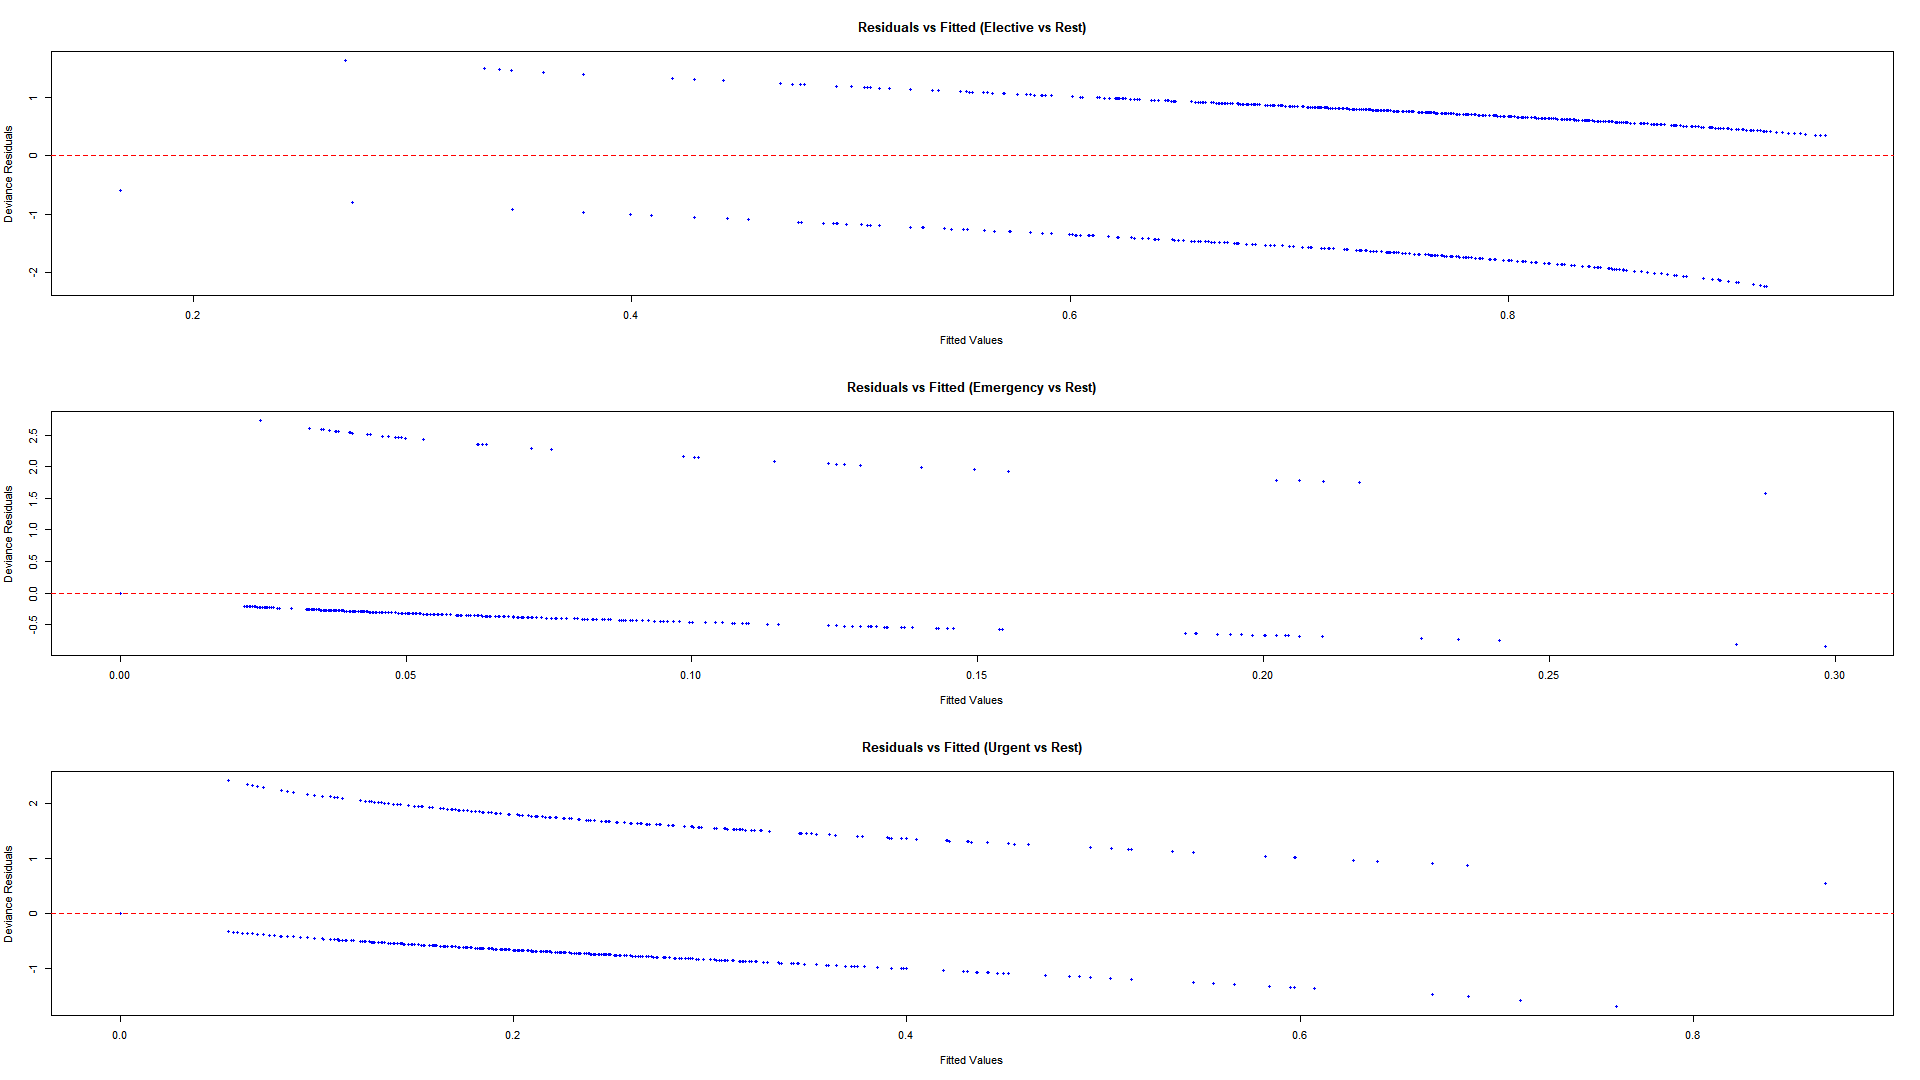
\includegraphics[width=\textwidth]{img/fitted_residuals_binomial.png}
    \caption{Fitted versus residuals plots for each binomial model. All models exhibit some parallel lines in the residuals plots suggesting model instability, but this effect is less prevelant in emergency vs rest compared to the other models.}
    \label{fig:fitted_residuals_binomial}
\end{figure}

\begin{table}[ht]
\centering
\begin{tabular}{lccc}
\hline
\textbf{Variable} & \textbf{Emergency} & \textbf{Urgent} & \textbf{Elective} \\
\hline
(Intercept) & 1.555994911 & -0.525044435 & -0.57200868 \\
los & 0.009673969 & 0.001039893 & 0.03975408 \\
died1 & 0.078621827 & 0.019627569 & 0.42034458 \\
has\_emergency1 & -1.475908153 & 0.043273349 & -1.18270522 \\
has\_urgent1 & 0.129361595 & 0.506774631 & 0.43362102 \\
has\_elderly1 & -0.098049243 & 0.009571130 & -0.64731587 \\
has\_youth1 & 0.258583369 & 0.048766229 & -1.20302056 \\
white1 & -0.121840658 & -0.003091603 & -0.47039122 \\
has\_pediatric1 & 0.123422552 & 0.040652210 & 0.52321164 \\
has\_emergency1:has\_youth1 & -0.222762934 & 0.074960221 & 1.62914321 \\
has\_elderly1:has\_youth1 & 0.066094317 & -0.082772564 & 0.26897299 \\
\hline
\end{tabular}
\caption{Coefficient differences between the multinomial model and the corresponding binomial model. The columns indicate how the multinomial coefficients for Emergency and Urgent admissions differ from their corresponding binomial model coefficients, while the Elective column reflects the difference from the baseline (0) in the multinomial model. The binomial models produce similar coefficients for demographic and case variables, but differs significantly for the admissions-based hospital dummy variables.}
\label{tab:coeff_differences}
\end{table}

\begin{figure}[ht]
    \centering
    \begin{subfigure}[b]{0.45\textwidth}
        \centering
        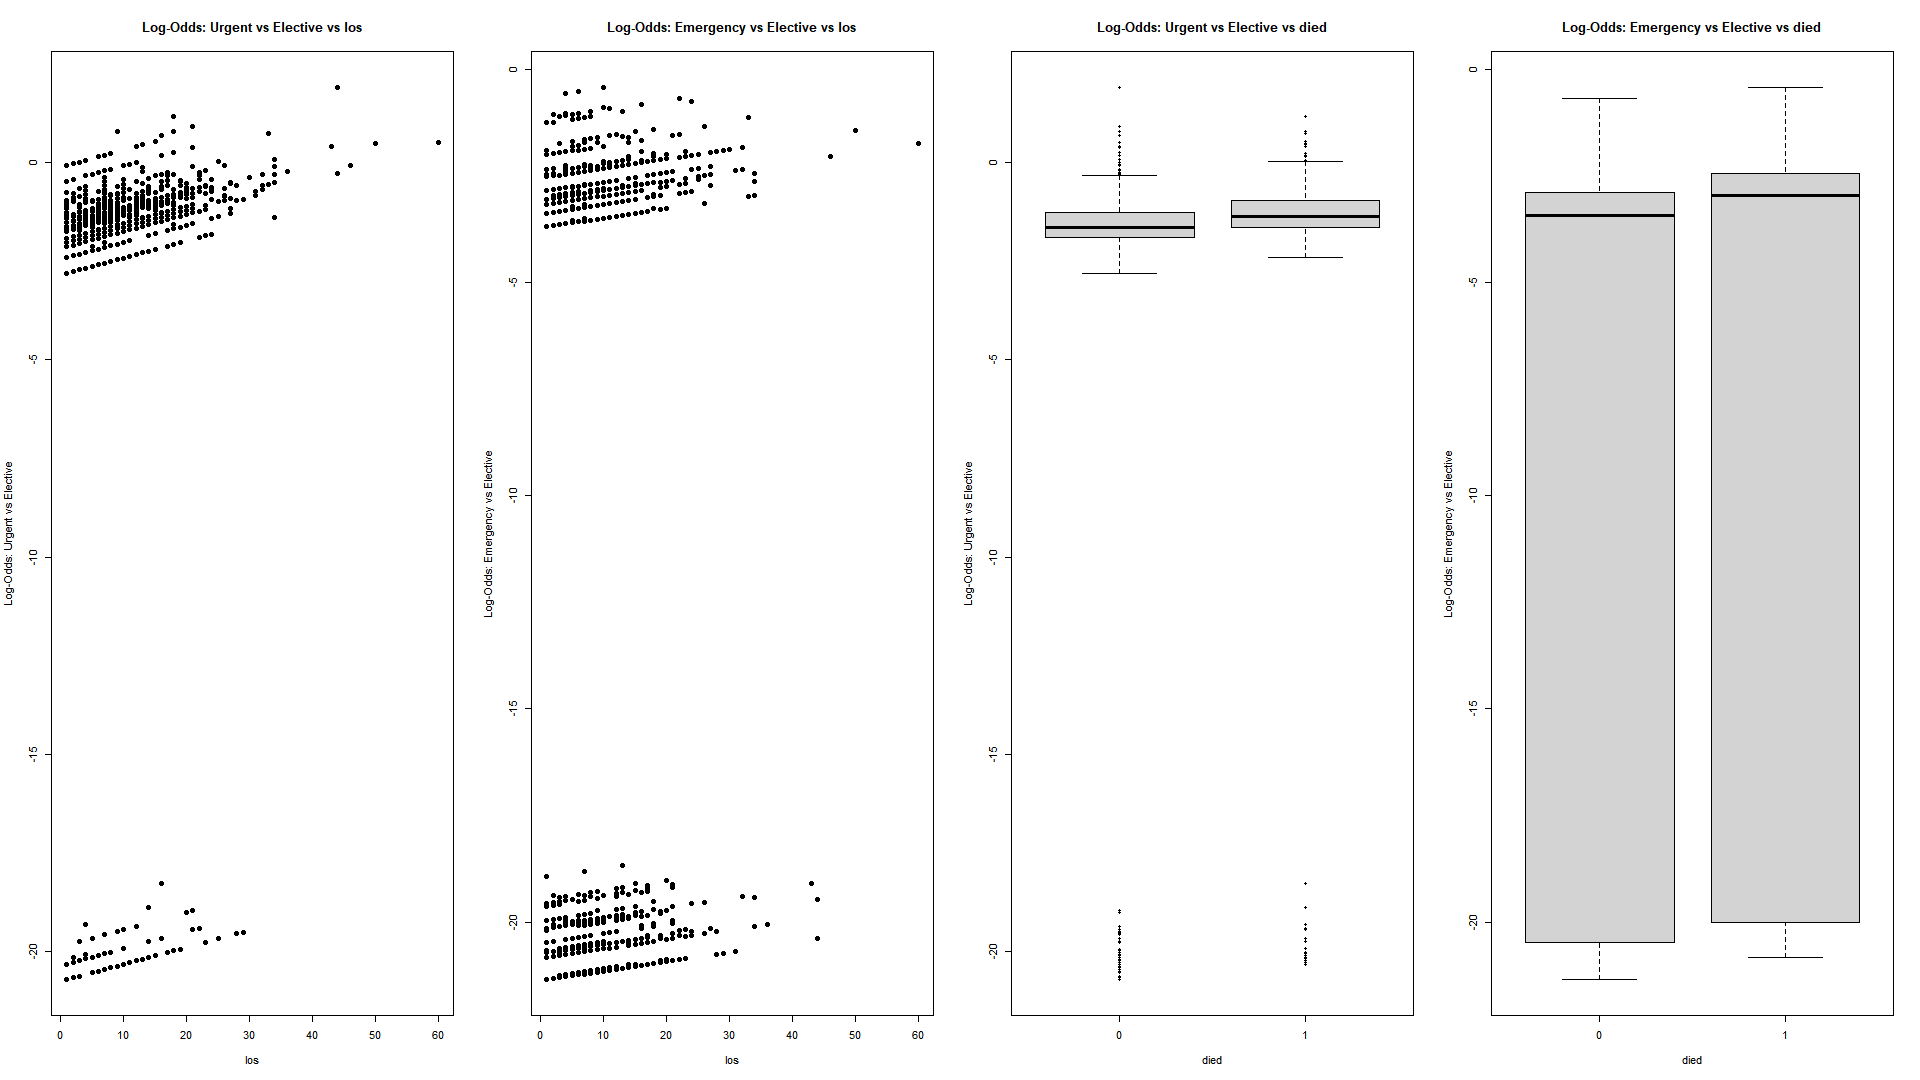
\includegraphics[width=\textwidth]{img/log_odds_1.png}
    \end{subfigure}
    \hfill
    \begin{subfigure}[b]{0.45\textwidth}
        \centering
        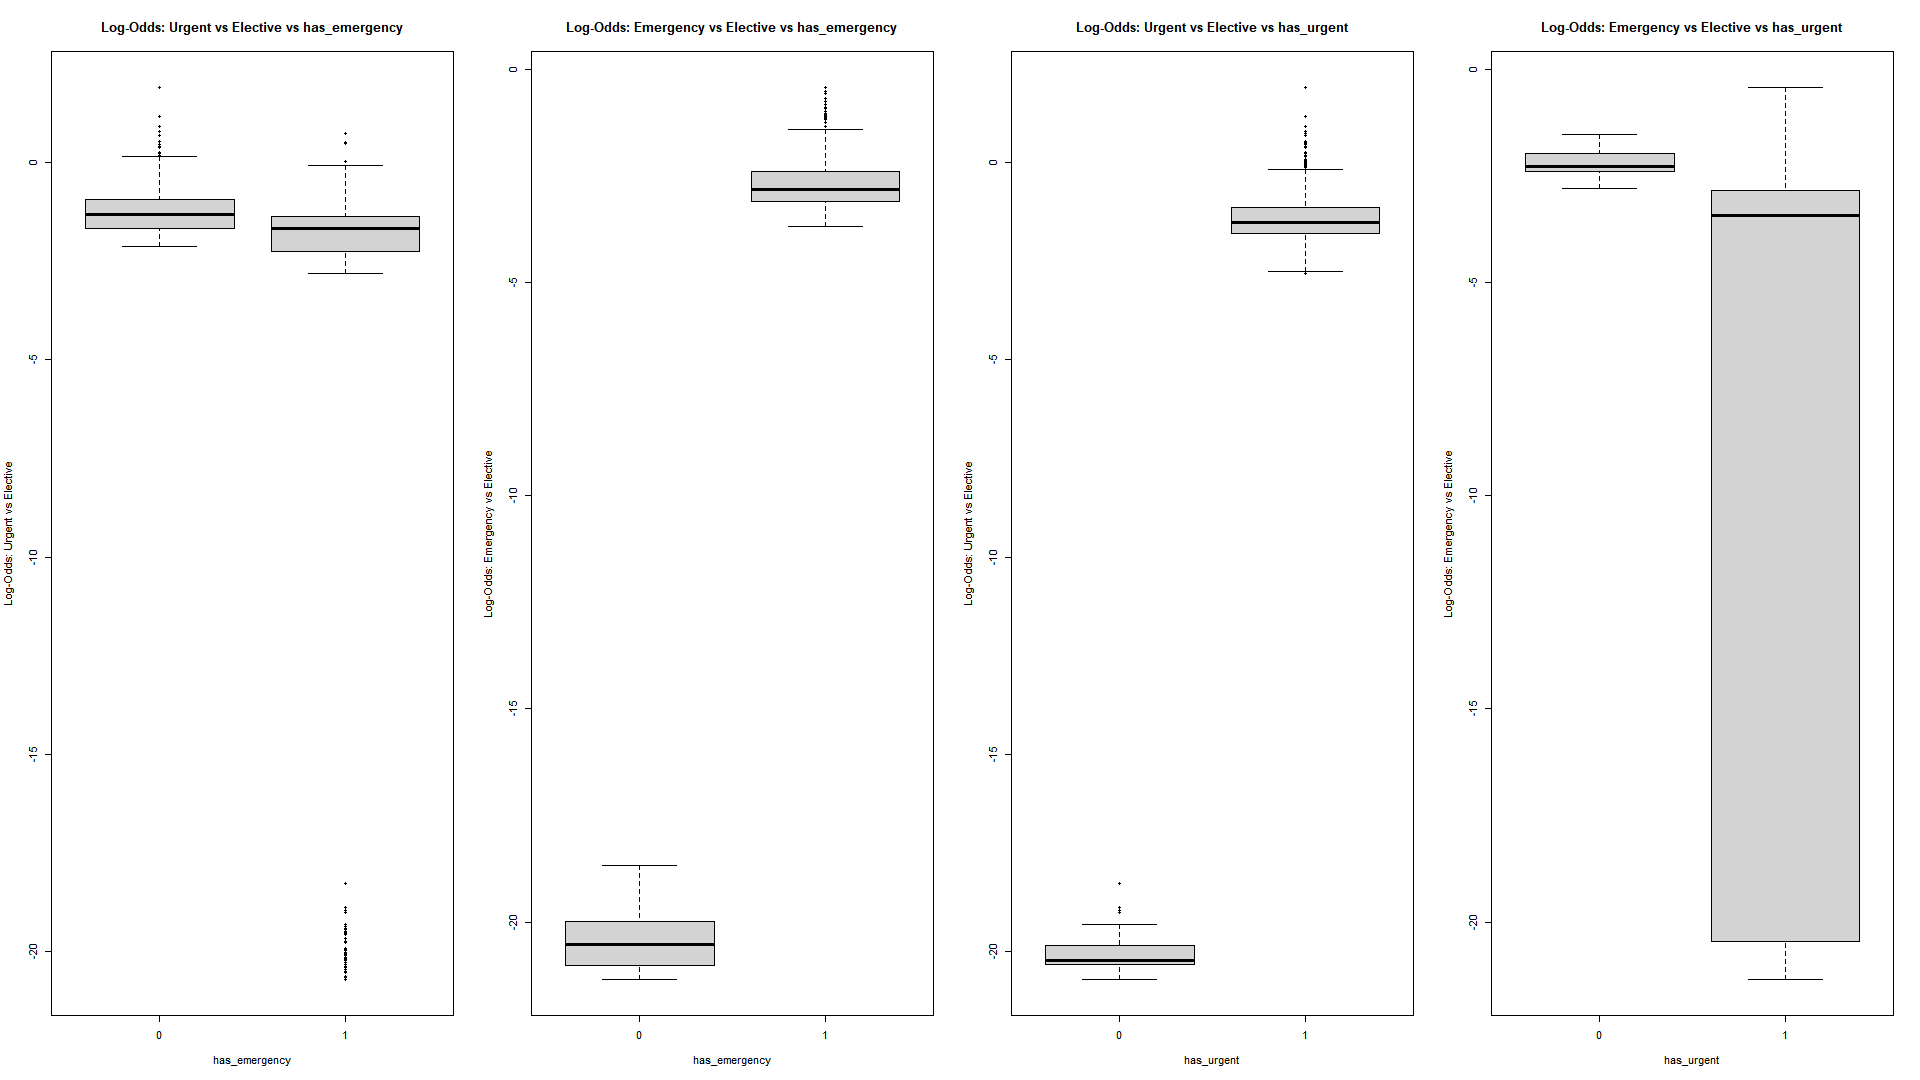
\includegraphics[width=\textwidth]{img/log_odds_2.png}
    \end{subfigure}

    \vspace{0.5cm}

    \begin{subfigure}[b]{0.45\textwidth}
        \centering
        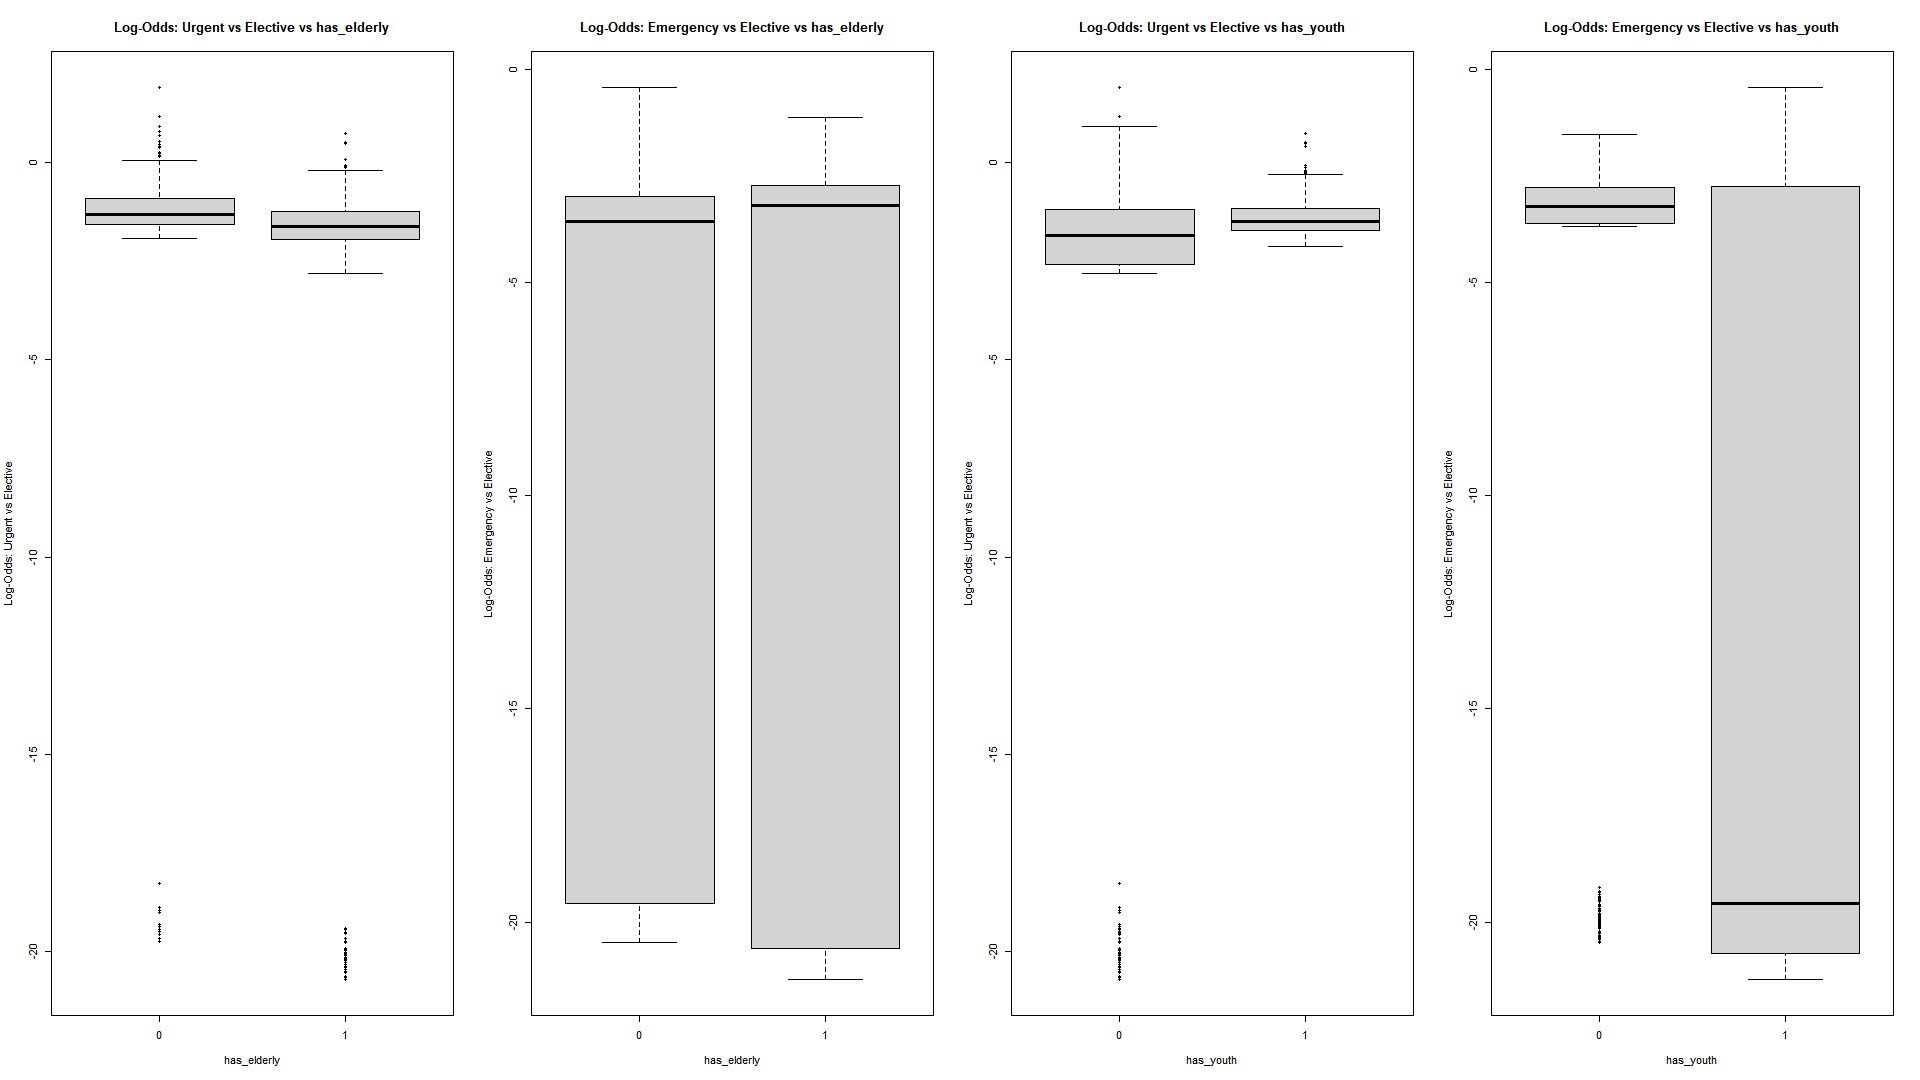
\includegraphics[width=\textwidth]{img/log_odds_3.png}
    \end{subfigure}
    \hfill
    \begin{subfigure}[b]{0.45\textwidth}
        \centering
        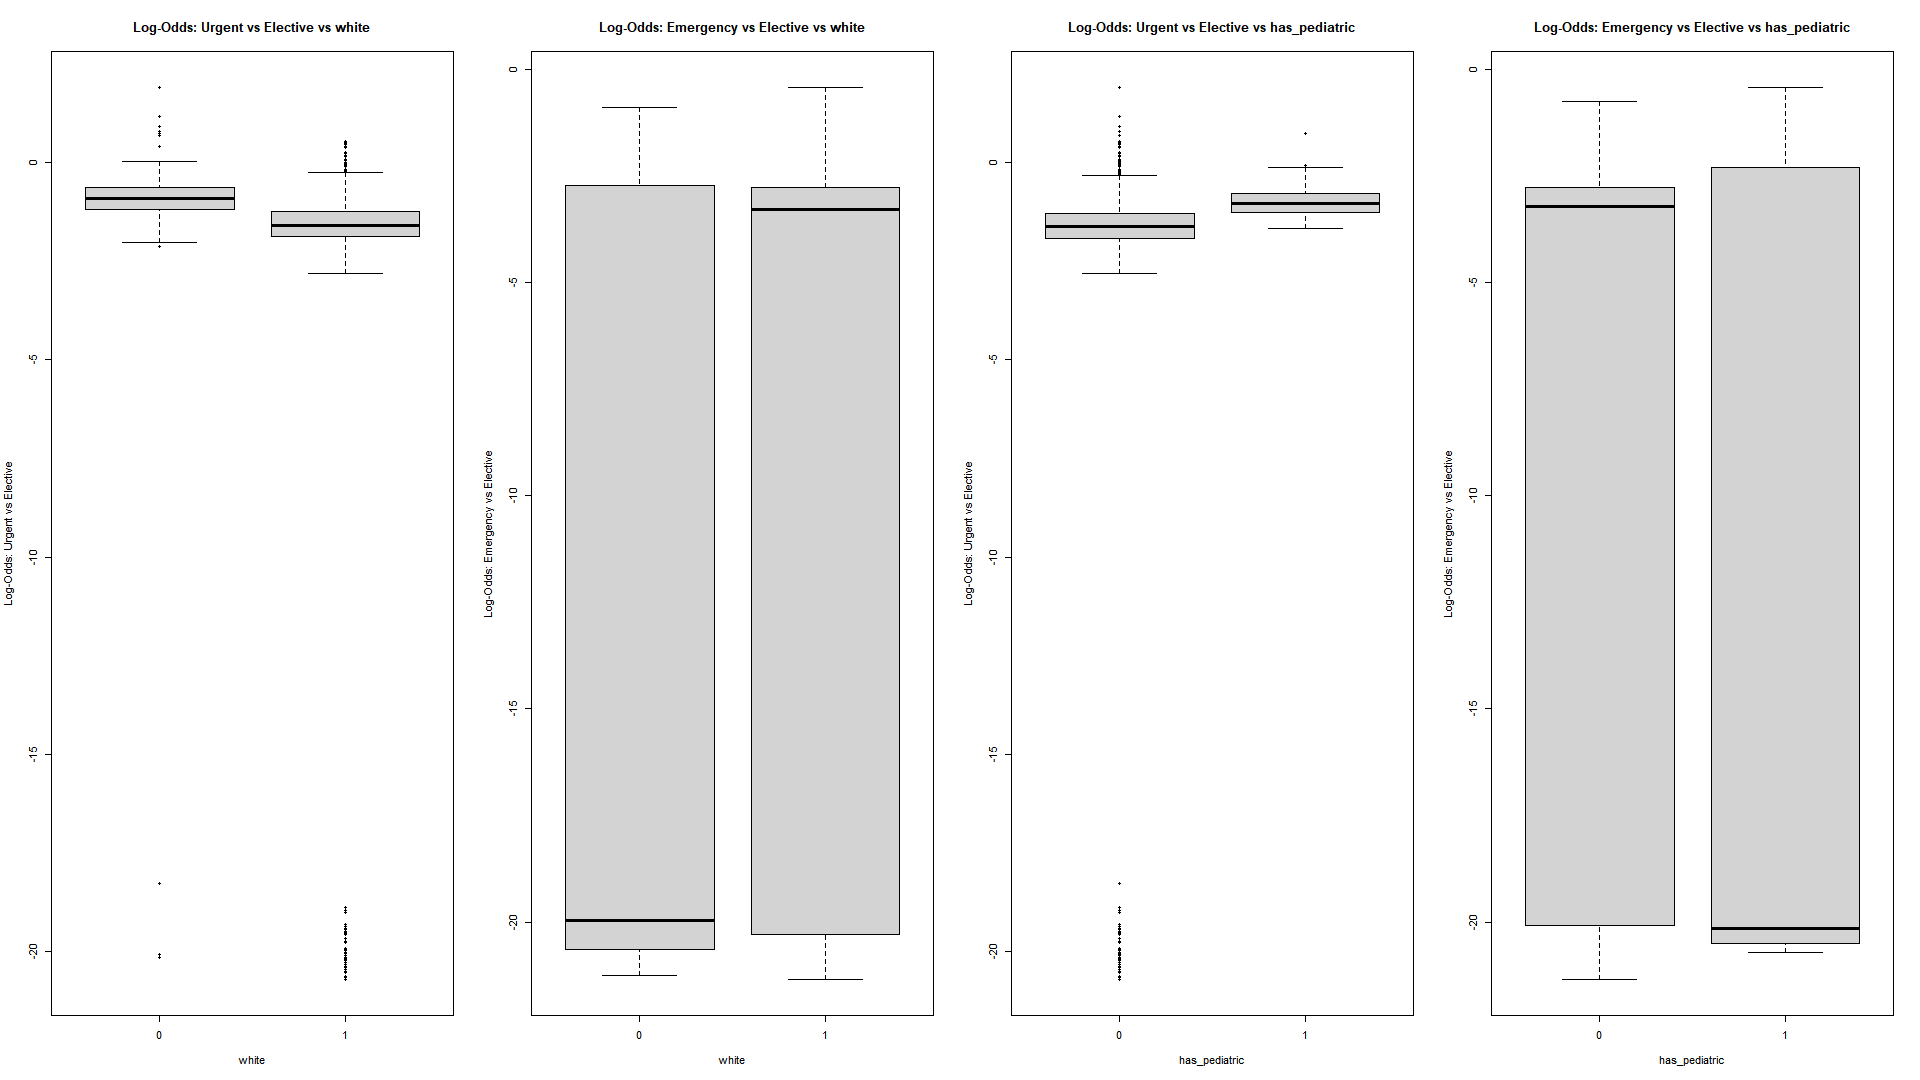
\includegraphics[width=\textwidth]{img/log_odds_4.png}
    \end{subfigure}

    \caption{Log-odds for admissions categories given the state of a particular predictor, assuming all other predictor coefficients are zero. Many of these factor variables (died, has\_elderly, has\_youth, white, has\_pediatric) have overlap between their baseline and activated states for both emergency and urgent. The only continuous variable (length of stay) exhibits a linear trend, with the banding reflecting an influence of another binary variable.}
    \label{fig:log_odds_grid}
\end{figure}

\begin{figure}[ht]
    \centering
    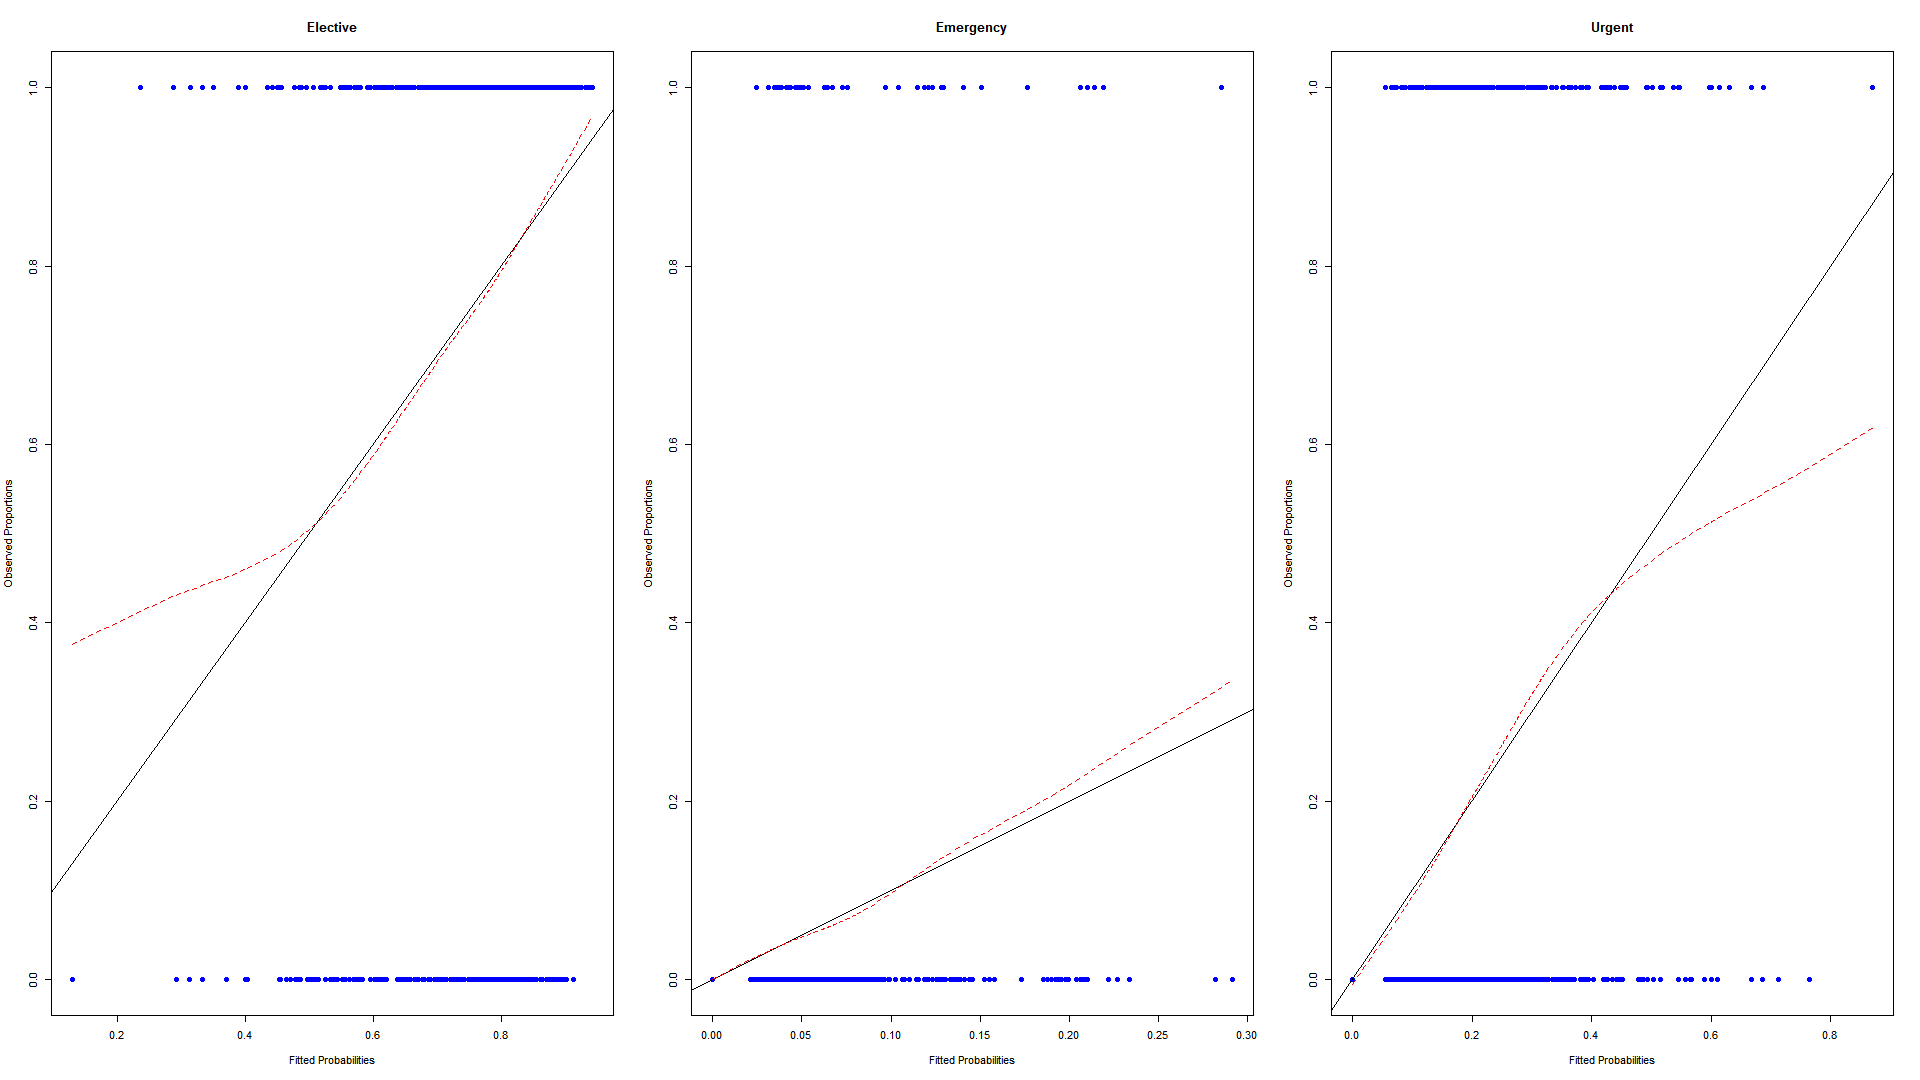
\includegraphics[width=\textwidth]{img/fitted_observed.png}
    \caption{Fitted versus observed values for the multinomial model. The deviations of the red spline from the black reference line shows that the model overestimates the odds of elective admissions at low predicted probabilities, overestimates the odds of emergency admissions at higher predicted probabilities, and underestimates the odds of urgent admissions at higher probabilities.}
    \label{fig:fitted_observed}
\end{figure}

\end{document}

